%%%%%%%%%%%%%%%%%%%%%%%%%%%%%%%%%%%%%%%%%%%%%%%%%%
% 配電網 例 (第1章で使う)
%%%%%%%%%%%%%%%%%%%%%%%%%%%%%%%%%%%%%%%%%%%%%%%%%%

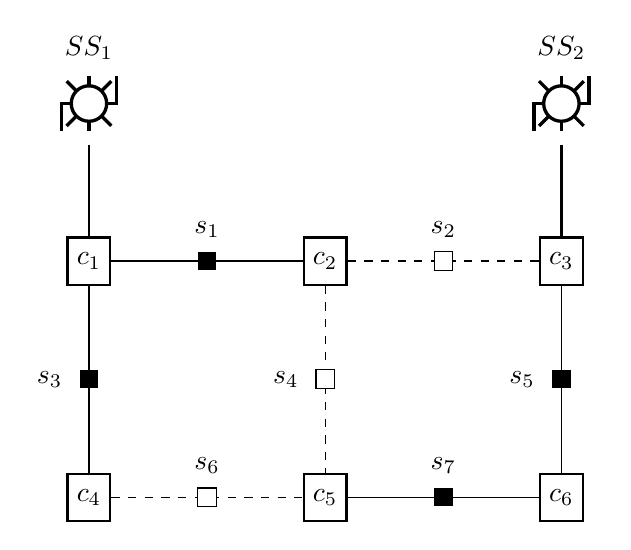
\begin{tikzpicture}

 % 設定
 \tikzset{customer/.style={rectangle,thick,draw=black,minimum height=0.6cm}}
 \tikzset{on_switch/.style={rectangle,fill=black}}
 \tikzset{off_switch/.style={rectangle,draw=black,fill=white}}

 % 補助線
 % \draw [help lines,blue,step=1cm] (-5,0) grid (5,-5);
  
 % substation1 (ホントはnewcommandでできるようにしたかった...)
 \draw [very thick] (-3,0) circle [radius=0.225cm] node[draw=white,minimum size=1cm](root1){};
 \draw [very thick] (-2.775,0)--(-2.65,0)--(-2.65,0.35);
 \draw [very thick] (-3.225,0)--(-3.35,0)--(-3.35,-0.35);
 \draw [very thick] (-3,0.225)--(-3,0.35);
 \draw [very thick] (-3,-0.225)--(-3,-0.35);
 \draw [very thick] [domain=-0.284:-0.159] plot(\x-3,\x);
 \draw [very thick] [domain=0.159:0.284] plot(\x-3,\x);
 \draw [very thick] [domain=-0.284:-0.159] plot(\x-3,-\x);
 \draw [very thick] [domain=0.159:0.284] plot(\x-3,-\x);
 \node at (-3,0.7) {$SS_{1}$};

 % substation2
 \draw [very thick] (3,0) circle [radius=0.225cm] node[draw=white,minimum size=1cm](root2){};
 \draw [very thick] (3.225,0)--(3.35,0)--(3.35,0.35);
 \draw [very thick] (2.775,0)--(2.65,0)--(2.65,-0.35);
 \draw [very thick] (3,0.225)--(3,0.35);
 \draw [very thick] (3,-0.225)--(3,-0.35);
 \draw [very thick] [domain=-0.284:-0.159] plot(\x+3,\x);
 \draw [very thick] [domain=0.159:0.284] plot(\x+3,\x);
 \draw [very thick] [domain=-0.284:-0.159] plot(\x+3,-\x);
 \draw [very thick] [domain=0.159:0.284] plot(\x+3,-\x);
 \node at (3,0.7) {$SS_{2}$};

 % 需要家 customer
 \node[customer] at (-3,-2)(1){$c_1$};
 \node[customer] at (0,-2) (2){$c_2$};
 \node[customer] at (3,-2) (3){$c_3$};
 \node[customer] at (-3,-5) (4){$c_4$};
 \node[customer] at (0,-5) (5){$c_5$};
 \node[customer] at (3,-5) (6){$c_6$};

 % 辺
 % ルート
 \draw [thick] (root1) -- (1);
 \draw [thick] (root2) -- (3);
 % 繋がってない辺は点線
 \foreach \u / \v in {2/3, 2/5, 4/5}
 \draw [dashed] (\u) -- (\v);
 % 繋がってる辺は実線
 \foreach \u / \v in {1/2, 1/4, 3/6, 5/6}
 \draw (\u) -- (\v);

 % スイッチ switch %
 % \node[on_switch] at (-3,-1) (s1){};
 % \node at (-3.5,-1) {$s_1$};
 %
 % \node[on_switch] at (3,-1) (s2){};
 % \node at (2.5,-1) {$s_2$};
 %
 \node[on_switch] at (-1.5,-2) (s1){};
 \node at (-1.5,-1.6) {$s_1$};
 %
 \node[off_switch] at (1.5,-2) (s2){};
 \node at (1.5,-1.6) {$s_2$};
 %
 \node[on_switch] at (-3,-3.5) (s3){};
 \node at (-3.5,-3.5) {$s_3$};
 %
 \node[off_switch] at (0,-3.5) (s4){};
 \node at (-0.5,-3.5) {$s_4$};
 %
 \node[on_switch] at (3,-3.5) (s5){};
 \node at (2.5,-3.5) {$s_5$};
 %
 \node[off_switch] at (-1.5,-5) (s6){};
 \node at (-1.5,-4.6) {$s_6$};
 %
 \node[on_switch] at (1.5,-5) (s7){};
 \node at (1.5,-4.6) {$s_7$};
 %

\end{tikzpicture}

%%%%%%%%%%%%%%%%%%%%%%%%%%%%%%%%%%%%%%%%%%%%%%%%%%%%%%%%%%
%%% Local Variables:
%%% mode: japanese-latex
%%% TeX-master: paper.tex
%%% End:
